\subsection{RQ4 --- Does the selective trigger work under live traffic?}
\label{sec:rq4}
Table~\ref{tab:stream} compares the policies at 75\% load on CIC-IDS2017, and Fig.~\ref{fig:stream:cic} shows all three loads.

\begin{table}[!htbp]
\centering
\caption{Explanation policies on CIC-IDS2017 at 75\% load. Overhead = explanation work as a share of detection time; Covered = share of true alerts with an exact explanation within 1\,s; Delay = 99th-percentile time to a verdict in seconds.}
\label{tab:stream}
\scriptsize
\setlength{\tabcolsep}{4pt}
\begin{minipage}[t]{0.495\textwidth}
\centering
\begin{tabular}{lrrr}
\toprule
\multicolumn{4}{c}{\textbf{Normal (mixed) traffic}} \\
\midrule
\textbf{Policy} & \textbf{Overhead} & \textbf{Covered} & \textbf{Delay (s)} \\
\midrule
B1 explain none & 0.00 & 0.00 & 0.003 \\
B2a all, TreeSHAP & 2.14 & 0.06 & 16.72 \\
B2b all, KernelSHAP & 257.67 & 0.00 & 2117.02 \\
B3 one global expl. & 0.00 & 0.00 & 0.058 \\
B4 random & 0.37 & 0.16 & 0.243 \\
B5 every alert & 0.13 & 1.00 & 0.008 \\
B6 learned explainer & 0.29 & 0.75 & 1.44 \\
\textbf{Proposed} & 0.11 & 1.00 & 0.032 \\
\bottomrule
\end{tabular}
\end{minipage}
\hfill
\begin{minipage}[t]{0.495\textwidth}
\centering
\begin{tabular}{lrrr}
\toprule
\multicolumn{4}{c}{\textbf{With port-scan flood}} \\
\midrule
\textbf{Policy} & \textbf{Overhead} & \textbf{Covered} & \textbf{Delay (s)} \\
\midrule
B1 explain none & 0.00 & 0.00 & 0.006 \\
B2a all, TreeSHAP & 2.15 & 0.01 & 18.68 \\
B2b all, KernelSHAP & 242.34 & 0.00 & 2435.23 \\
B3 one global expl. & 0.00 & 0.00 & 0.004 \\
B4 random & 0.60 & 0.03 & 2.58 \\
B5 every alert & 0.42 & 0.41 & 2.68 \\
B6 learned explainer & 0.29 & 1.00 & 0.670 \\
\textbf{Proposed} & 0.10 & 1.00 & 0.035 \\
\bottomrule
\end{tabular}
\end{minipage}
\end{table}


\begin{itemize}[leftmargin=*, itemsep=0pt]
  \item \textbf{Explaining every flow is impossible.} With TreeSHAP it costs 2.1 times the detection time, so verdicts are delayed by 17--19\,s; with KernelSHAP it costs about 250 times. The learned explainer (B6) is cheaper (0.29) but still delays verdicts by 0.7--1.4\,s, and its explanations differ from exact TreeSHAP.
  \item \textbf{In normal traffic, explaining every alert (B5) is affordable} (overhead 0.13, delay 8\,ms). The trigger also explains every alert within 1\,s (57\% instantly) at overhead 0.106 and a 32\,ms delay. On top of that it explains uncertain flows, which include 20 of the 22 attacks the detector missed.
  \item \textbf{During the flood, only the trigger stays fast.} B5's overhead rises to 0.42 and its delay to 2.7\,s, and only 41\% of alerts are explained in time. The trigger keeps overhead at 0.105 and delay at 35\,ms and explains every alert within 1\,s, because flood flows are near-copies and the cache answers 61\% of requests. Cached explanations are as good as fresh ones (faithfulness 0.563 vs.\ 0.575).
  \item \textbf{At overload (150\%)} no policy keeps up. The trigger pauses explanation and stays at the explain-nothing delay (2.7--3.1\,s).
  \item \textbf{Limit:} one core of KernelSHAP finishes about 9 explanations per second, so on CIC-IDS2017 only 24--26\% of the deep requests finish within 30\,s.
  \item \textbf{HIKARI shows the same pattern:} overhead 0.101--0.102, every alert explained within 1\,s, and a delay of 5--19\,ms, against 318\,ms for B5 during the flood.
\end{itemize}
\textbf{H4 is supported within detection capacity:} the overhead is 0.101--0.106 (the 10\% budget plus a small burst allowance), all true alerts are explained within 1\,s, and the delivered explanations are statistically equivalent in quality to fresh exact ones (TOST, margin 0.05).

\begin{figure}[!htbp]
\centering
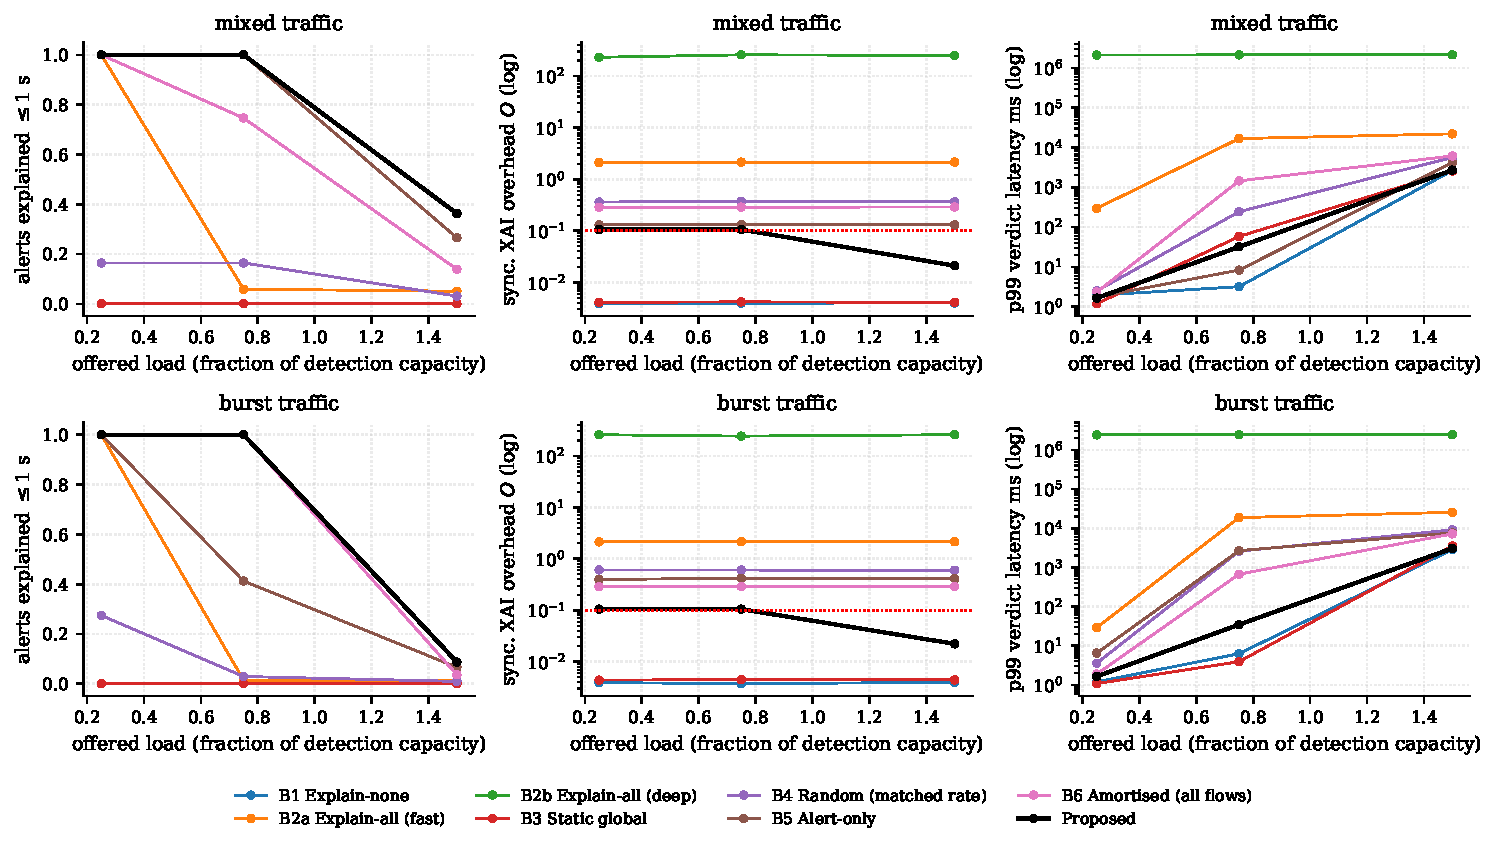
\includegraphics[width=\textwidth]{../figures/fig_stream_cic2017_XGB_T3.pdf}
\caption{CIC-IDS2017, XGBoost on $T_3$: alerts explained within 1\,s (left), explanation overhead (middle; dotted line = 10\% budget) and 99th-percentile verdict delay (right) against load, for normal (top) and flood (bottom) traffic.}
\label{fig:stream:cic}
\end{figure}
